\section{Ohjelmistojen testaaminen ja mobiilisovellusten testaamisen erityispiirteitä}

Tässä luvussa esitellään ohjelmistojen testauksen peruskäsitteitä, testauksen asemaa ohjelmistotuotantoprosessissa, mobiilisovellusten testaamisen erityispiirteitä sekä pohditaan, miten testaustyökaluja voi arvioida.

\subsection{Testaamisen peruskäsitteitä}

Testitapaus (\emph{test case}) on yksittäinen testi, jolle on määritelty syötteet, suoritusehdot ja läpäisykriteerit. Testisarja (\emph{test suite}) taas on joukko testitapauksia. Testisarja voi myös koostua useasta testisarjasta, jolloin esimerkiksi ohjelman jokaiselle komponentille voi olla oma testisarjansa ja yksi testisarja kattaa sitten kaikki yksittäisten komponenttien testisarjat \cite[153]{testing}.

Yksikkötestaus on useimmiten lasilaatikkotestausta (\emph{white box testing} / \emph{structural testing} / \emph{glass box testing}), jolloin testejä voidaan kirjoittaa ohjelmakoodin perusteella. Testeiltä voidaan vaatia esimerkiksi tiettyä koodikattavuutta, jolloin varmistetaan, että mahdollisimman suuri osa ohjelmakoodista tulee suoritettua testien aikana \cite[154]{testing}.

Toiminnallisessa testauksessa (\emph{functional testing}) testattavan ohjelman sisäistä rakennetta ei tunneta, vaan ollaan kiinnostuneita vain syötteistä ja niitä vastaavista tulosteista. Toiminnallista testausta voidaan kutsua myös musta laatikko -testaukseksi (\emph{black box testing}). Toiminnallisessa testauksessa ollaan kiinnostuneita ohjelman käyttäjälle näkyvästä toiminnasta, ja testejä voidaan tehdä esimerkiksi ohjelman määrittelyn pohjalta \cite[161-162]{testing}.

Fuzz-testaus on satunnaistestauksen muoto, jossa ohjelmaan kohdistetaan satunnaisia syötteitä ja seurataan ohjelman tulosteita. Syötteitä voidaan myös luoda kielioppien avulla, jolloin voidaan käyttää hyödyksi tietoa testattavasta ohjelmasta. Fuzz-testaus on osoittautunut tehokkaaksi tavaksi löytää sovelluksista virheitä, joita muut testaustavat eivät paljasta. Toisaalta satunnaisuus tarkoittaa, että testejä pitää suorittaa lukemattomia kertoja, jos fuzz-testaukselle halutaan kattava testipeitto. Fuzz-testaus on havaittu erityisen tehokkaaksi turvallisuusaukkoja etsittäessä \cite{fuzztesting}.

Jäljittely (\emph{mocking}) on tekniikka, joka helpottaa yksikkötestien kirjoittamista. Yksikkötestien ulkoiset riippuvuudet voidaan korvata testeissä kontrolloitavilla jäljittelijäolioilla. Tällöin testit ovat vakaampia, koska ulkopuolisten komponenttien muokkaus ei vaikuta testeihin, testin haluttuun lopputulokseen vaikuttava ympäristö on helppo saada haluttuun muotoon. Tällöin testien on helppo testata myös sellaisia olosuhteita, jotka ovat harvinaisia tai vaikeita saada muokattua. Lisäksi jäljittelemällä voidaan korvata vielä toteuttamattomat ulkoiset riippuvuudet jäljittelijätoteutuksilla \cite{mocking}.

\subsection{Testaaminen osana ohjelmistotuotantoprosessia}

\begin{figure}[h]
\centering
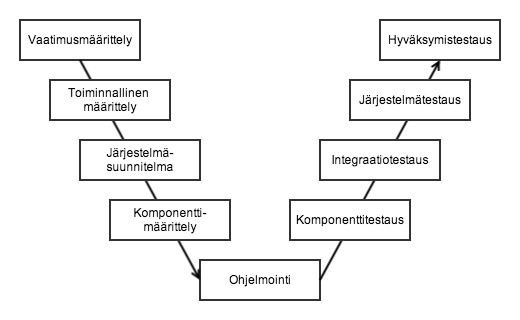
\includegraphics[width=140mm]{v_malli.png}
\caption{Testauksen v-malli \protect\cite[40]{testing_foundations}} \label{v_model}
\end{figure}

Ohjelmistotuotantoprosessia lähestytään yleensä jonkin elinkaarimallin kautta. Testauksen näkökulmaa edustaa testauksen v-malli, joka on esitetty kuvassa \ref{v_model}. Mallin yleisessä versiossa lähdetään siitä, että jokaista ohjelmistotuotantoprosessin vaihetta vastaa jokin testausvaihe. Näin testaus tehdään ohjelmistotuotantoprosessissa näkyväksi ja yhtä tärkeäksi osaksi kuin itse sovelluksen kehittäminen. Kuvassa v:n vasemmalla haaralla on vesiputousmallin mukaiset ohjelmistotuotantoprosessin vaiheet. Ensimmäisenä vaiheena on vaatimusmäärittely. Tässä vaiheessa määritellään loppukäyttäjän tai asiakkaan tarpeet ja vaatimukset sovellukselle.  Viimeinen vaihe on alimpana oleva sovelluksen ohjelmointi. Oikealla haaralla ovat testausvaiheet, joissa jokaisessa varmistetaan, että ohjelma täyttää vasemman haaran samalla tasolla olevassa vaiheessa suunnitellut vaatimukset \cite[39-42]{testing_foundations}.

V-mallin alimmalla tasolla on komponentti- eli yksikkötestaus. Siinä testataan ohjelman pienempiä itsenäiseen toimintaan kykeneviä osasia, eli olio-ohjelmoinnin tapauksessa useimmiten luokkia. Android-sovellusten tapauksessa tällä voidaan ajatella yksittäistä Android-komponenttia, esimerkiksi aktiviteettia, tai jopa aktiviteettia pienempiä osia, kuten yksittäistä näkymä-luokkaa tai muuta toimintaa tarjoavaa alikomponenttia. Komponenttitestaus on useimmiten valkoinen laatikko -testausta ja sen suorittaminen vaatii ohjelmointitaitoa. Useimmiten sovelluksen ohjelmoijat suorittavat itse komponenttitestauksen. Komponenttitestauksella pyritään varmistamaan, että komponentti täyttää sen toiminnallisen määritelmän. Komponenttitestejä tehdään usein eri kielille kehitetyillä automaattisilla yksikkötestikehyksillä, kuten Javan JUnitilla. Oikean toiminnallisuuden testaamisen lisäksi on tärkeää testata myös toiminta väärillä syötteillä ja poikkeustilanteissa. Moderni tapa tehdä komponenttitestausta on kirjoittaa testikoodi ennen sovelluskoodia \cite[43-50]{testing_foundations}.

V-mallin seuraavalla tasolla on integraatiotestaus. Siinä vaiheessa oletetaan, että komponenttitestaus on jo tehty ja yksittäisten komponenttien omaan toimintaan liittyvät virheet on löydetty. Integraatiovaiheessa yksittäisten komponentit yhdistetään toisiinsa ja testataan, että niiden yhteistoiminta on oikeanlaista. Tavoitteena on löytää mahdolliset virheet komponenttien rajapinnoista ja komponenttien välisestä yhteistyöstä. Testauksessa voidaan käyttää apuna tynkiä (\emph{stub}) sellaisista komponenteista, jotka eivät vielä ole valmiita \cite[50-52]{testing_foundations}.

V-mallin kolmannella testaustasolla on järjestelmätestaus (\emph{system testing}). Järjestelmätestauksessa testataan, että täysin integroitu järjestelmä toimii kokonaisuutena kuten pitäisi. Alemmista tasoista poiketen järjestelmätestauksessa näkökulma on järjestelmän tulevan käyttäjän, kun alemmilla tasoilla testaus on luonteeltaan enemmän teknistä. Järjestelmätestauksessa varmistetaan, että järjestelmä kokonaisuudessaan täyttää sille asetetut toiminnalliset ja ei-toiminnalliset vaatimukset. Järjestelmätestauksessa ei tulisi käyttää enää tynkiä, vaan järjestelmän kaikki komponentit tulisi asentaa esimerkiksi erilliseen testiympäristöön testausta varten. Itse sovelluksen lisäksi järjestelmätestauksen piiriin kuuluvat ohjelmiston dokumentaatio ja konfiguraatio \cite[58-61]{testing_foundations}.

V-mallin viimeinen vaihe on hyväksyntätestaus. Alemmilla tasoilla sovellus on ollut kehittäjän vastuulla, mutta hyväksyntätestauksessa järjestelmä testataan asiakkaan näkökulmasta. Tällöin pyritään varmistamaan, että tuotettu järjestelmä täyttää mahdollisen toimitussopimuksen ja sen käyttäjät hyväksyvät järjestelmän. Hyväksyntätestaus voi sisältää myös alfa tai beta -testauksen oikeilla järjestelmän loppukäyttäjillä \cite[62-63]{testing_foundations}.

Testauksen jokaisessa vaiheessa ollaan kiinnostuneita validoinnista ja verifioinnista. Validoinnissa varmistetaan, että toteutus täyttää järjestelmän alkuperäisen tehtävän, eli että rakennetaan oikeaa sovellusta. Verifioinnissa taas varmistetaan, että kehitysvaiheessa tuotettu sovelluksen osa vastaa sille tehtyä spesifikaatiota, eli että sovellus on tehty oikein. V-mallin eri vaiheissa validoinnin ja verifikaation painotukset vaihtelevat. Alemman tason testauksessa on kyse enemmän verifikaatiosta ja ylemmän tason testauksessa taas validoinnista \cite[41-42]{testing_foundations}.

Automaattiset testityökalut ovat tyypillisesti sitä enemmän käytössä, mitä alemmalla v-mallin testaustasolla testausta tehdään. Varsinkin komponenttitestaus on tyypillisesti täysin automatisoitua. Testauksen automatisoinnilla pyritään testausprosessin tehostamiseen, kun testien suorittaminen on nopeaa. Lisäksi testien luotettavuus paranee, kun epäluotettavat manuaaliset vaiheet korvataan automaattisilla \cite[201]{testing_foundations}.

\subsection{Mobiilisovellusten testaamisen erityispiirteitä}

Mobiilisovellusten kehittämiseen liittyy haasteita, jotka liittyvät mobiiliympäristön rajoituksiin. Näitä ovat muun muassa päätelaitteiden rajallinen kapasiteetti ja jatkuva kehittyminen, erilaiset standardit, protokollat ja verkkotekniikat, päätelaitteiden monimuotoisuus, mobiililaitteiden käyttäjien erikoistarpeet sekä tiukat aikavaatimukset sovellusten saamiseksi markkinoille. Sovellusmarkkinat ovat myös globaalit, joten sovellusten lokalisoinnissa eri kieli- ja kulttuuriympäristöihin aiheuttaa haasteita.

Sovelluksia rajoittaa myös mobiililaitteiden pieni fyysinen koko ja laitteiden erot koossa, painossa ja näytön koossa. Myös käyttöliittymissä on eroja, joskin kosketusnäyttöpuhelimet ovat vallanneet suurimman osan markkinoista viime vuosina.

Mobiilisovelluksen on oltava laadultaan hyvä, jotta se on helppo saada toimimaan oikein erilaisissa laiteympäristöissä. Lisäksi julkaisunopeus voi olla kriittinen tekijä markkinaosuuden valtaamisessa. Jos kilpaileva sovellus julkaistaan viikkoa aikaisemmin, voi markkina olla jo täytetty sovelluksen julkaisuhetkellä.

VTT on kehittänyt mobiilisovellusten kehittämiseen ketterän Mobile-D-lähestymistavan. Testauksen kannalta olennaista on testilähtöisen kehityksen käyttäminen (\emph{test driven development}, \emph{tdd}). Mobile-D:hen kuuluu testien kirjoittaminen ennen tuotantokoodin kirjoitusta, yksikkötestien automatisointi ja kaikkien ominaisuuksien hyväksyntätestaus asiakkaan kanssa \cite{abrahamsson04}.

Testilähtöisessä kehityksessä on kaksi merkittävää periaatetta: ohjelmakoodia saa kirjoittaa vain automaattisen testin korjaamiseksi ja duplikaattikoodin poistamiseksi. Näistä periaatteista seuraa tunnettu tdd-sykli: punainen, vihreä, refaktoroi. Ensin kirjoitetaan testi, joka ei mene läpi, koska testin toteuttavaa ohjelmakoodia ei ole vielä olemassa. Vaiheen nimi on punainen, koska useimmilla yksikkötestityökaluilla lopputuloksena näkyy punainen palkki, jos jokin testi ei mene läpi. Toinen vaihe on kirjoittaa juuri sen verran koodia, mitä tarvitaan testin läpäisemiseksi. Tässä vaiheessa ei välitetä miten luettavaa ja eleganttia koodi on. Vaiheen nimi on vihreä, koska useimmissa yksikkötestityökaluissa lopputuloksena näkyy vihreä palkki, kun testit menevät läpi. Viimeisessä vaiheessa refaktoroidaan toisessa vaiheessa mahdollisesti syntynyt duplikaatti- tai muuten vaikealukuinen koodi. Testit auttavat varmistamaan, ettei refaktoroidessa hajoiteta vanhaa toiminnallisuutta. Jotta tällainen ohjelmointisykli olisi mahdollinen, ohjelmistoympäristön täytyy tarjota mahdollisuus saada nopeasti palaute pienestä testijoukosta, jottei ohjelmoidessa jouduta jatkuvasti odottamaan testien ajautumista \cite{tdd}.

\subsection{Testityökalujen arviointikriteereistä}
\label{test_criteria}

Androidille on tehty Androidin mukana tulevien testaustyökalujen lisäksi monia muita testaustyökaluja. Nämä työkalut erottautuvat Androidin työkaluista joko pyrkimällä toteuttamaan jonkin asian paremmin kuin vastaava Androidin oma testaustyökalu tai sitten tarjoamalla testaamiseen sellaisen lähestymistavan, jota Androidin omat testaustyökalut eivät tarjoa.

Testaustyökalujen arviointia käsittelevät muun muassa Poston ja Sexton \cite{poston92}. Hyvän testaustyökalun kriteerit ovat osin kontekstista riippuvia, mutta Poston ja Sexton määrittelevät myös yleisempiä kriteerejä testityökalujen arviointiin. Usein kriteerit ovat myös helposti määriteltävissä: jollain työkalulla pystyy testaamaan asioita, joita toisella ei voi. Ei-toiminnallisista olennaisista ominaisuuksista he luettelevat työkalun tehokkuuden, miten nopeasti sen käytön oppii, miten nopeaa testien tekeminen sillä on ja miten luotettava työkalu on.

Michael et al. \cite{michael02} ovat kehittäneet joukon metriikoita testityökalun tehokkuuden arviointiin. Heidän käyttämänsä metriikat ovat saaneet innoituksensa tavallisille sovelluksille kehitetyistä erilaisista kompleksisuusmetriikoista, kuten koodirivien määrä tai syklomaattinen kompleksisuus. He esittävät listan vastaavia metriikoita testityökalujen tehokkuuden arviointiin. Näitä arvoja voi sitten painottaa testityökalujen valinnassa haluamallaan tavalla. Metriikoita ovat muun muassa työkalun kypsyys ja käyttäjäkunnan koko, helppokäyttöisyys, kustomointimahdollisuudet, automaattinen testitapausten generointi, muiden ohjelmointityökalujen tarjoama tuki työkalulle, luotettavuus sekä suoritusnopeus. Osalle metriikoista esitetään myös täsmällisiä laskukaavoja, jotka helpottavat kvantitatiivisen analyysin tekemistä.

Spillner et al. \cite[218]{testing_foundations} listaavat testityökalujen valintaan vaikuttavia tekijöitä:
\begin{itemize}
  \itemsep0em
  \item Miten hyvin testityökalu saa tietoa ja pystyy vaikuttamaan testattavaan sovellukseen
  \item Testaajien tietotaito työkalun käytöstä
  \item Miten hyvin työkalu voidaan integroida käytössä oleviin kehitystyökaluihin
  \item Miten hyvin työkalu voidaan integroida muihin käytettäviin testaustyökaluihin
  \item Millä alustalla työkalu toimii
  \item Työkalun valmistajan tarjoama tuki, luotettavuus ja markkina-asema
  \item Lisenssiehdot, hinta ja ylläpitokustannukset
\end{itemize}

Osa kriteereistä on hyvin kontekstiriippuvaisia, mutta myös niitä voi soveltaa yleisemmän arvioinnin tekemisessä. Esimerkiksi testaajien tietotaidon sijaan voidaan arvioida, miten helppoa työkalun käyttö on oppia.